\hypertarget{part-1-design-5}{%
\section{Part 1, design 5}\label{part-1-design-5}}

\begin{figure}
\centering
%\includegraphics{pathtofigure.png}
\caption{Design 5}
\end{figure}

\centering
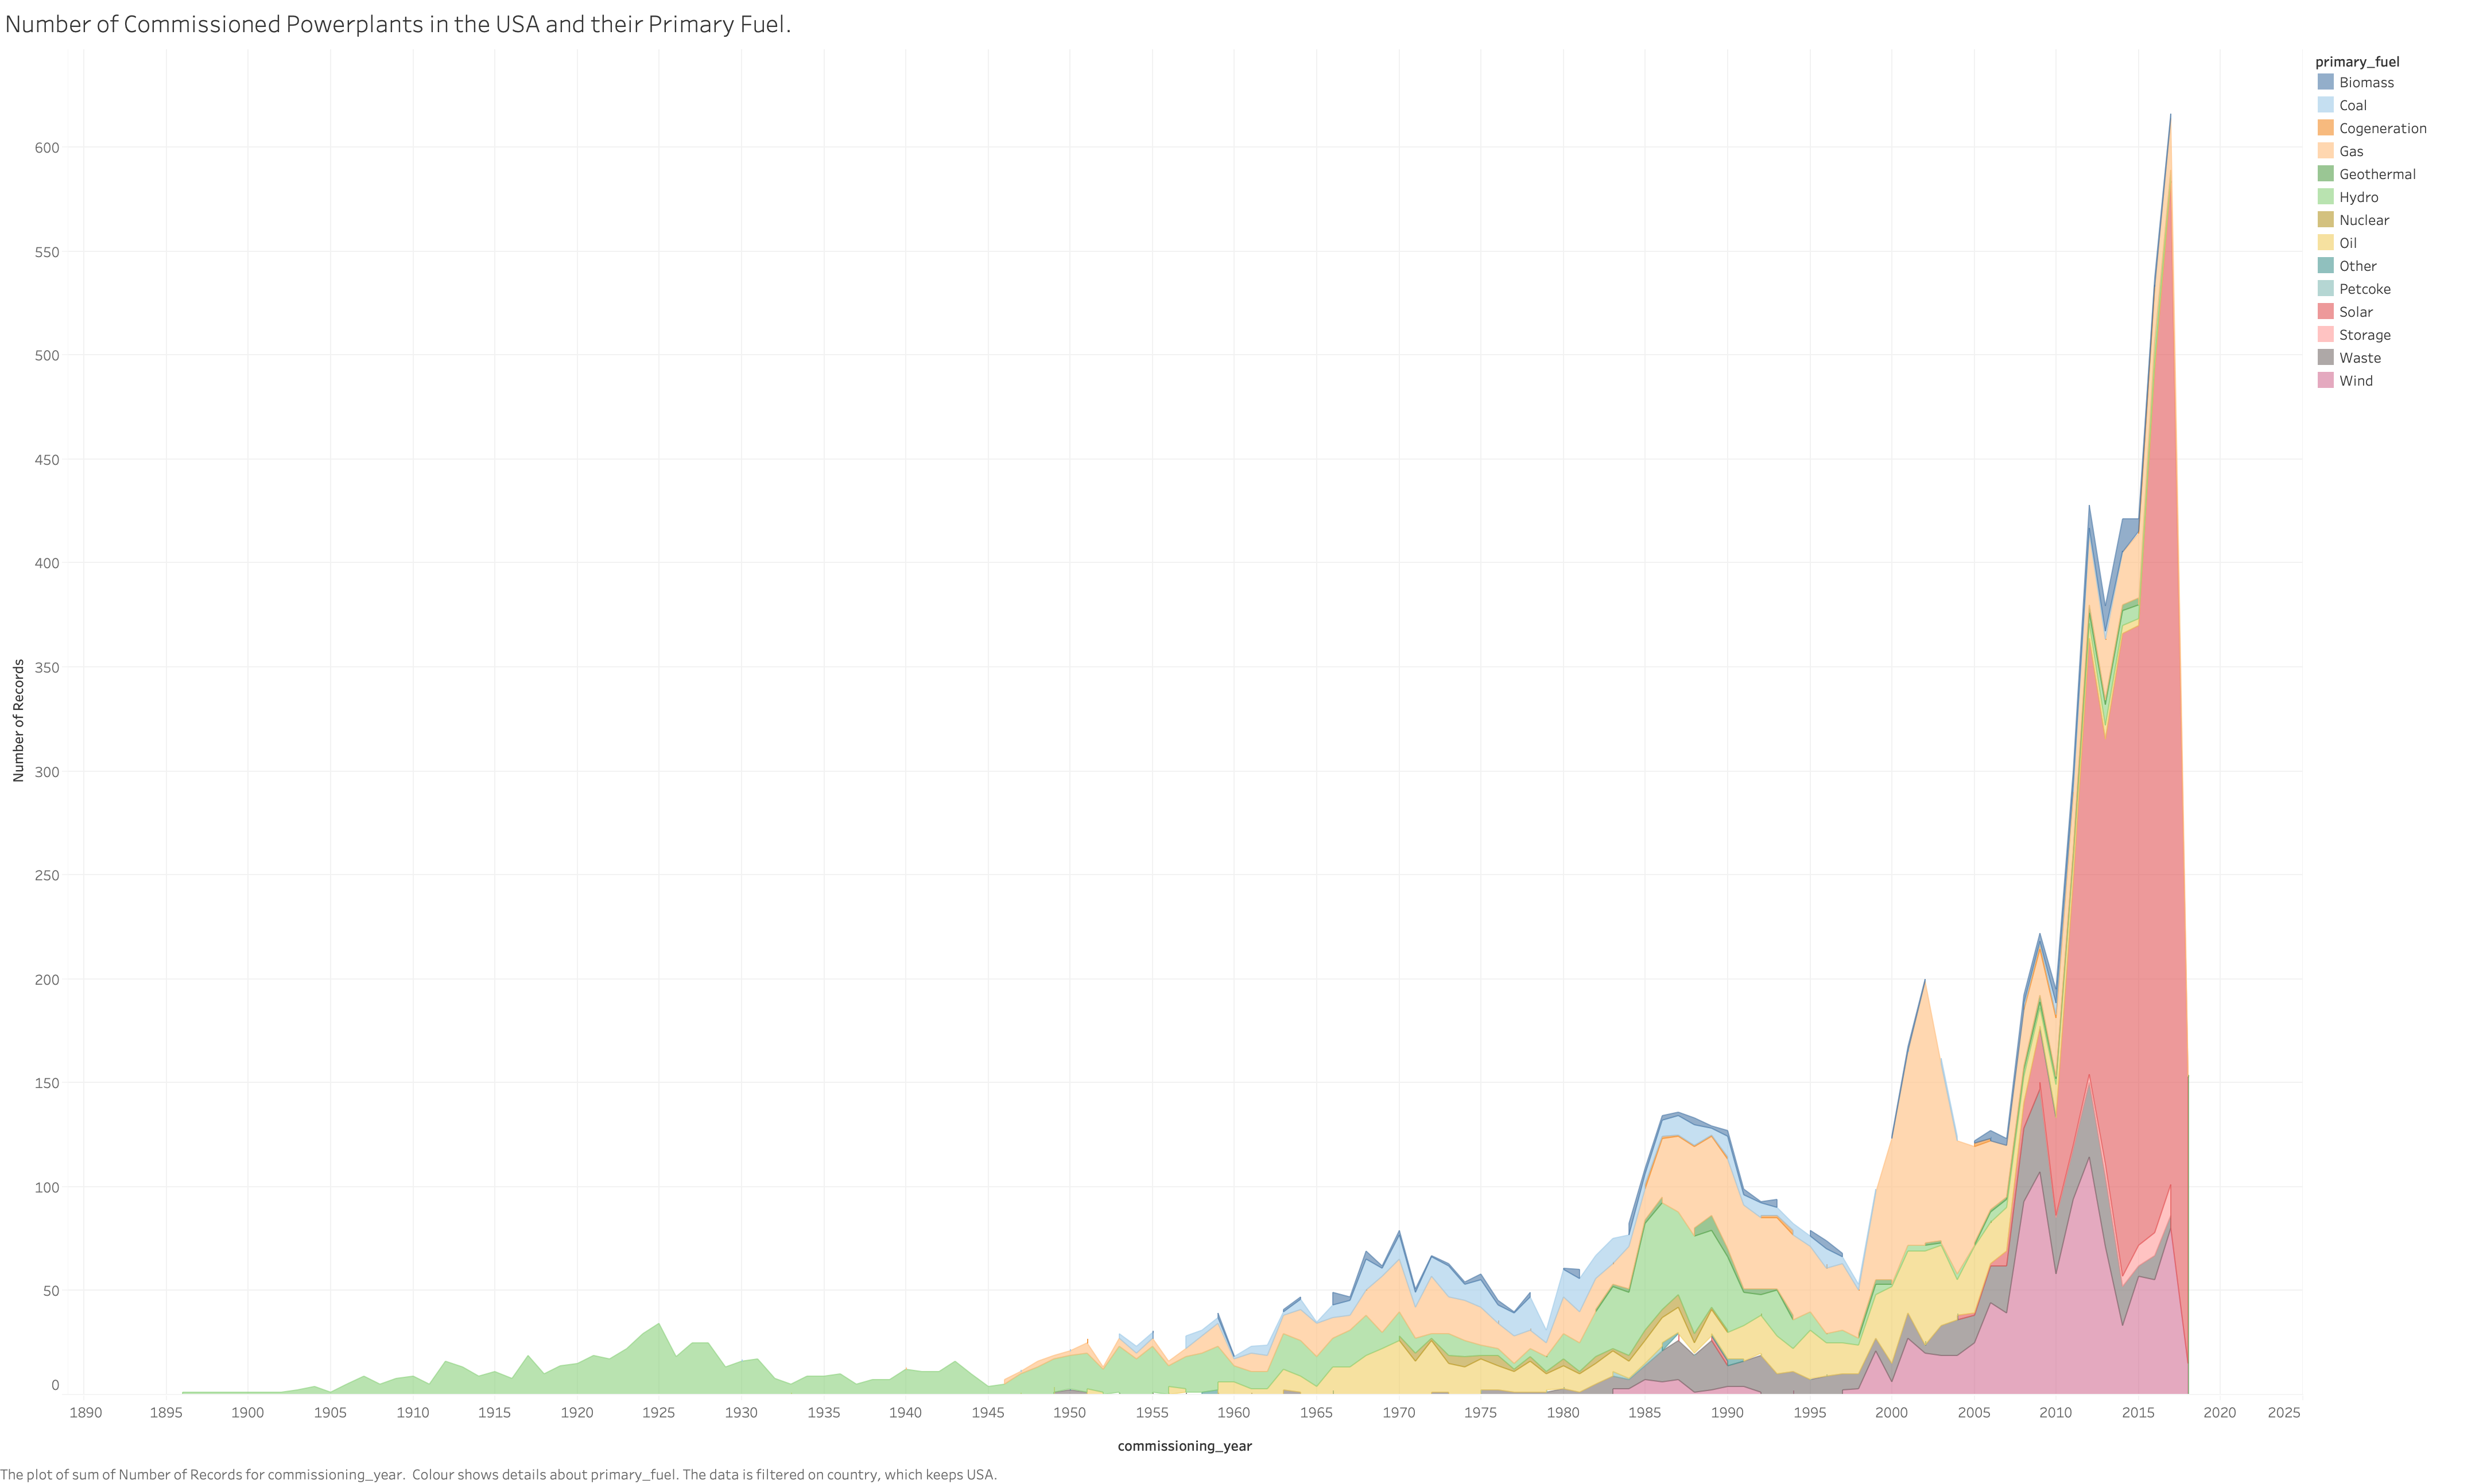
\includegraphics[width=15cm]{Viz5.png}

\hypertarget{description}{%
\subsubsection{Description}\label{description}}

\begin{description}
\item[Visual Design Type:]
Area Charts Continuous.
\item[Name of Tool:]
Tableau
\item[Country:]
USA
\item[Year:]
1890 - 2018
\item[Visual Mappings:]
\begin{itemize}
\tightlist
\item
  \textbf{mapping 1}: ???
\end{itemize}

\begin{itemize}
\tightlist
\item
  \textbf{mapping 2}: ???
\end{itemize}
\item[Unique Observation:]
???
\item[Data Preparation:]
No alterations.
\end{description} 
